%==============================常用宏包、环境==============================%
\documentclass[landscape,twocolumn,twoside,a4paper]{article}
\usepackage{xeCJK} % For Chinese characters
\usepackage{amsmath, amsthm}
\usepackage{listings,xcolor}
\usepackage{geometry} % 设置页边距
\usepackage{fontspec}
\usepackage{graphicx}
\usepackage{fancyhdr} % 自定义页眉页脚
\usepackage{makecell}
\usepackage[breaklinks,colorlinks,linkcolor=black,citecolor=black,urlcolor=black]{hyperref}
\setsansfont{Consolas} % 设置英文字体
\setmonofont[Mapping={}]{Consolas} % 英文引号之类的正常显示,相当于设置英文字体
\geometry{left=1.5cm,right=1cm,top=1.5cm,bottom=0.5cm} % 页边距
% \setlength{\columnsep}{15pt}
% \setlength\columnseprule{0.4pt} % 分割线

\usepackage{xunicode, xltxtra} 
\setmainfont{Microsoft YaHei} 
\usepackage{setspace}
\usepackage{ctex} 
\usepackage[Glenn]{fncychap}
\usepackage{color}
\usepackage{verbatim}
\usepackage{titlesec}
\usepackage{markdown}


%==============================常用宏包、环境==============================%
\newfontfamily\monaco{Monaco}
\definecolor{dkgreen}{rgb}{0,0.6,0}
\definecolor{gray}{rgb}{0.5,0.5,0.5}
\definecolor{mauve}{rgb}{0.58,0,0.82}

%==============================页眉、页脚、代码格式设置==============================%
% 页眉、页脚设置

\pagestyle{fancy}
\fancyhead{} %clear all fields
\fancyhead[RO]{\CJKfamily{hei} 第 \thepage 页} %奇数页眉的右边
\fancyhead[LE]{\CJKfamily{hei} 第 \thepage 页} %奇数页眉的右边
% \lhead{CUMTB}
% \lhead{\CJKfamily{hei} Standard Code Library}
% \chead{}
% \rhead{Page \thepage}
% \rhead{\CJKfamily{hei} 第 \thepage 页}
% \lfoot{} 
% \cfoot{}
% \rfoot{\CJKfamily{hei} 第 \thepage 页}
\renewcommand{\headrulewidth}{0.4pt} 
\renewcommand{\footrulewidth}{0.4pt}

% \lstset{
%     language    = c++,
%     numbers     = left,
%     numberstyle = \tiny,
%     breaklines  = true,
%     captionpos  = b,
%     tabsize     = 4,
%     frame       = simple,
%     columns     = fullflexible,
%     commentstyle = \color{gray},
%     keywordstyle = \bfseries\monaco,
%     basicstyle   = \monaco,
%     stringstyle  = \color[RGB]{148,0,209}\ttfamily,
%     rulesepcolor = \color{red!20!green!20!blue!20},
%     showstringspaces = false,
% }

\lstset{
    frame = simple,
    language = c++,
    aboveskip = 3mm,
    belowskip = 3mm,
    showstringspaces = false,
    basicstyle = \monaco,
    numbers = left,
    numberstyle = \tiny\color{gray},
    keywordstyle = \bfseries\monaco,%\fontspec{monaco Bold}\bfseries,
    commentstyle = \color{gray},
    stringstyle = \color{mauve},
    breaklines = true,
    breakatwhitespace = true,
    tabsize = 4
}

%==============================页眉、页脚、代码格式设置==============================%

%==============================标题和目录==============================%
% \title{\CJKfamily{hei} \bfseries Standard Code Library}
% \author{Xavier\_Cai}
% \renewcommand{\today}{\number\year 年 \number\month 月 \number\day 日}

\begin{document}\small
% \begin{titlepage}
% \maketitle
% \end{titlepage}

\newpage
\pagestyle{empty}
\renewcommand{\contentsname}{目录}
\tableofcontents
\newpage\clearpage
\newpage
\pagestyle{fancy}
\setcounter{page}{1}   %new page

%==============================基本操作=============================%
\section{基本操作}

\subsection{快读fread}
\lstinputlisting{杂项/fread.cpp}

\subsection{朝鲜人快读}
\lstinputlisting{基本操作/朝鲜人快读.cpp}

\subsection{\_\_int128}
\lstinputlisting{其它/__int128.cpp}

\subsection{二维离散化}
\subsubsection{基本操作/离散化/二维点离散化.cpp}

\subsection{矩阵快速幂}
\lstinputlisting{基本操作/矩阵.cpp}

\subsection{状态压缩}
\lstinputlisting{基本操作/状态压缩.cpp}

\subsection{二进制枚举}
\lstinputlisting{基本操作/二进制枚举.cpp}

\subsection{bitset}
\lstinputlisting{基本操作/bitset.cpp}

\subsection{高效位运算 \_\_builtin\_ 函数}
\lstinputlisting{基本操作/高效位运算.cpp}

\subsection{散列处理异或碰撞}
\lstinputlisting{其它/散列处理异或碰撞.cpp}

\subsection{对拍}
\lstinputlisting{其它/对拍.cpp}


%==============================STL=============================%
\section{STL}

\subsection{unordered\_map对pii进行哈希}
\lstinputlisting{STL/unordered_map对pii进行哈希.cpp}

\subsection{pb\_ds实现平衡树}
\lstinputlisting{STL/pb_ds实现平衡树.cpp}

\subsection{rope}
写一种数据结构,支持任意位置插入、删除和修改
\lstinputlisting{STL/rope.cpp}


%==============================数论=============================%
\section{数论}

\subsection{中国剩余定理}
$\left\{\begin{matrix} x \equiv a_{1} (\mod m_{1})\\ x \equiv a_{2} (\mod m_{2})\\  x \equiv a_{3} (\mod m_{3})\\  x \equiv a_{4} (\mod m_{4})\end{matrix}\right.$ \par
其中,$m_1,m_2,...,m_k$为两两互质的整数
\lstinputlisting{yx数论/中国剩余定理.cpp}

\subsection{蔡勒公式(1582之后)}
\lstinputlisting{数学/蔡勒公式(1582之后).cpp}

%==============================字符串=============================%
\section{字符串}

\subsection{字符串哈希}
\subsubsection{区间一维哈希}
\lstinputlisting{字符串/Hash/Hash.cpp}
% \subsubsection{二维哈希}
% \lstinputlisting{}



\subsection{Next函数}

\subsubsection{求next函数}
\lstinputlisting{字符串/Next函数/求next函数.cpp}

\subsubsection{求出每个循环节的数量和终点位置(HDU1358)}
\lstinputlisting{字符串/Next函数/求出每个循环节的数量和终点位置(HDU1358).cpp}

\subsubsection{求同时是前缀和后缀的串长(POJ2752)}
\lstinputlisting{字符串/Next函数/求同时是前缀和后缀的串长(POJ2752).cpp}

\subsubsection{求字符串每个前缀和串匹配成功的次数和(HDU3336)}
\lstinputlisting{字符串/Next函数/求字符串每个前缀和串匹配成功的次数和(HDU3336).cpp}

\subsubsection{求循环节数量(POJ2406)}
\lstinputlisting{字符串/Next函数/求循环节数量(POJ2406).cpp}

\subsubsection{求第一个串的前缀和第二个串的后缀的最大匹配(HDU2594)}
\lstinputlisting{字符串/Next函数/求第一个串的前缀和第二个串的后缀的最大匹配(HDU2594).cpp}

\subsubsection{求补上最少字母数量使得这是个循环串(HDU3746)}
\lstinputlisting{字符串/Next函数/求补上最少字母数量使得这是个循环串(HDU3746).cpp}

\subsubsection{习题整理}
\textbf{[NOI2014]动物园}\par
对于字符串$S$的前i个字符构成的子串,既是它的后缀同时又是它的前缀,并且该后缀与该前缀不重叠,将这种字符串的数量记作$num[i]$.\par
$res$为$(num[i]+1)$的乘积.\par
时间复杂度:$O(n).$
\lstinputlisting{字符串/Next函数/习题整理.cpp}

\subsection{KMP}

\subsubsection{统计模式串出现次数,出现位置,前缀border长度}
\lstinputlisting{字符串/KMP/统计模式串出现次数,出现位置,前缀border长度.cpp}

\subsubsection{矩阵加速KMP,求长度为n的不包含长度为m的子串的串个数([HNOI2008]GT考试)}
$$\sum_{k=0}^{m-1}f[i-1][k]\ast g[k][j]$$\par
$f[i][j]$ 为长串匹配到第$i$位,短串最多可以匹配到第$j$位的方案数\par
$g[j][k]$ 为了计算长度为$j$的已经匹配好了的串可以用多少种数字变为$k$,枚举一个数字,看它在短串中最长可以匹配到最多多长的前缀\par
\lstinputlisting{字符串/KMP/矩阵加速KMP([HNOI2008]GT考试).cpp}

\subsection{EXKMP}

\subsubsection{求z函数和LCP}
$LCP$:最长公共前缀\par
$z$函数数组$z$:串$b$与$b$的每一个后缀的$LCP$长度。\par
$extend$数组:串$b$与串$a$的每一个后缀的$LCP$长度。
总时间复杂度:$O(|a|+|b|)$.
\lstinputlisting{字符串/EXKMP/求z函数和LCP.cpp}

\subsubsection{循环位移有多少数比原数大小相等,去重(HDU4333)}
包含对获得的串进行去重。\par
总时间复杂度:$O(n)$
\lstinputlisting{字符串/EXKMP/循环位移有多少数比原数大小相等,去重(HDU4333).cpp}

\subsubsection{选出$n × n$对并把每一对连接成一个单词求回文对数(POJ3376)}
\lstinputlisting{字符串/EXKMP/例题.cpp}


\subsection{AC自动机}

\subsubsection{标准的AC自动机}
\lstinputlisting{字符串/AC自动机.cpp}

\subsubsection{AC自动机上检查无限长循环串([POI2000]病毒)}
\lstinputlisting{字符串/AC自动机上检查无限长循环串([POI2000]病毒).cpp}

\subsubsection{AC自动机+矩阵快速幂}
有 $m$ 种DNA序列是致病的,问长为 $n$ 且不包含致病序列的DNA有多少种\par
设 $dp[i][j]$ 为走了$j$ 步到达节点 $i$ 的方案数,显然 $dp[0][0]=1$,当 $i \neq 0$ 时,$dp[i][0]=0$。\par
设 $a[i][j]$ 为从节点 $i$ 到达节点 $j$ 是否存在边。\par
最终得 $dp[i][j] = \sum_{x=0}^{N} a[x][i] * dp[x][j-1]$\par
\lstinputlisting{字符串/AC自动机_矩阵快速幂.cpp}

\subsection{字典树/Trie树}
\lstinputlisting{字符串/Trie字典树.cpp}

\subsection{后缀数组SA}

\subsubsection{获取SA和rank数组}
\lstinputlisting{字符串/后缀数组/get_SA.cpp}

\subsubsection{后缀数组+ST表求lcp}
\lstinputlisting{字符串/后缀数组/后缀数组+ST表求lcp.cpp}

\subsubsection{后缀链接字典序最小(arc050\_d)}
\lstinputlisting{字符串/后缀数组/习题整理/后缀连接字典序最小(arc050_d).cpp}

\subsection{后缀自动机SAM}

\subsubsection{后缀自动机板子}
\textbf{应用1:不同子串个数}\par
给一个字符串$S$,计算不同子串的个数。\par
解法:利用后缀自动机的树形结构。每个节点对应的不同子串数量(不同位置算作同一个)是$maxlen[i]-maxlen[link[i]]$。\par
总时间复杂度:$O(|S|)$.\par
\textbf{应用2:所有不同子串的总长度}\par
给定一个字符串$S$,计算所有不同子串的总长度。
解法:利用上述后缀自动机的树形结构。每个节点对应的所有后缀长度是$\frac{maxlen[i]\ast (maxlen[i]+1)}{2}$,减去其$linke$节点的对应值$\frac{maxlen[link[i]]\ast (maxlen[link[i]]+1)}{2}$就是该节点的净贡献
\lstinputlisting{字符串/后缀自动机SAM/后缀自动机SAM.cpp}

\subsubsection{每个子串在多少个主串中出现过(SPOJ8093)}
暴力跳Link链.\par
时间复杂度:$均摊O(\sum |S|\sqrt{\sum |S|})$
\lstinputlisting{字符串/后缀自动机SAM/每个子串在多少个主串中出现过(SPOJ8093).cpp}

\subsubsection{第k小字串}
\lstinputlisting{字符串/后缀自动机SAM/第k小字串(不同位置的相同子串算作一个&多个)([TJOI2015]弦论).cpp}

\subsubsection{字典树建后缀自动机}
\lstinputlisting{字符串/后缀自动机SAM/字典树建后缀自动机.cpp}

\subsubsection{暴力在线统计出现次数为k次的字符串个数(HDU4641)}
\lstinputlisting{字符串/后缀自动机SAM/暴力在线统计出现次数为k次的字符串个数(HDU4641).cpp}


\subsection{Manacher}
\subsubsection{字符串/带条件的马拉车.cpp}

\subsection{回文自动机PAM}
\lstinputlisting{字符串/回文自动机/回文自动机PAM.cpp}


\subsection{序列自动机([HEOI2015]最短不公共子串)}
时间复杂度:$O(n|\sum|)$,其中$|\sum|$为字符集大小
\lstinputlisting{字符串/序列自动机.cpp}

\subsection{最小表示法}
时间复杂度:$O(n)$
\lstinputlisting{字符串/最小表示法.cpp}

\subsection{Lyndon分解}
将字符串分成若干部分$s = s_{1}s_{2}s_{3}...s_{m}$,使得每个$s_{i}$都是$Lyndon Word$。\par
$Lyndon Word$:当且仅当$s$是其所有后缀中最小字符串。
\lstinputlisting{字符串/Lyndon分解.cpp}

%==============================数据结构=============================%

\section{数据结构}

\subsection{ST表}
\lstinputlisting{数据结构/ST表.cpp}


\subsection{树状数组}

\subsubsection{lowbit之和}
\lstinputlisting{数据结构/树状数组/lowbit之和.cpp}

\subsubsection{区间加减+区间和查询}
\lstinputlisting{数据结构/树状数组/区间加减&区间和查询.cpp}

\subsubsection{统计前后顺序不同数字对个数(三维偏序问题)}
\lstinputlisting{数据结构/树状数组/统计前后顺序不同数字对个数(三维偏序问题).cpp}


\subsection{二维树状数组}

\subsubsection{单点修改+区间查询}
\lstinputlisting{数据结构/二维树状数组/单点修改+区间查询.cpp}

\subsubsection{区间修改+单点查询}
\lstinputlisting{数据结构/二维树状数组/区间修改+单点查询.cpp}

\subsubsection{区间修改+区间查询}
\lstinputlisting{数据结构/二维树状数组/区间修改+区间查询.cpp}


\subsection{线段树}


\subsubsection{单点修改+区间查询}
\lstinputlisting{数据结构/线段树/普通线段树/单点修改&区间查询.cpp}

\subsubsection{区间修改+区间查询}
\lstinputlisting{数据结构/线段树/普通线段树/区间修改&区间查询.cpp}

\subsubsection{区间染色}
\lstinputlisting{数据结构/线段树/普通线段树/区间染色.cpp}

\subsubsection{区间修改+区间查询:矩阵}
\lstinputlisting{数据结构/线段树/普通线段树/区间修改&区间查询_矩阵ver.cpp}

\subsubsection{区间中所有元素都严格出现三次的区间个数(CF1418G)}
\lstinputlisting{数据结构/线段树/普通线段树/区间中所有元素都严格出现三次的区间个数(CF1418G).cpp}

\subsubsection{线段树分裂合并}
\lstinputlisting{数据结构/线段树/普通线段树/线段树分裂合并.cpp}

\subsubsection{单点修改+单点最大连通数(HDU1540)}
\lstinputlisting{数据结构/线段树/普通线段树/单点修改单点最大连通个数.cpp}

\subsubsection{找到最前的长度为k的序列}
\lstinputlisting{数据结构/线段树/普通线段树/区间第一次出现长度为k位置.cpp}

\subsection{二维线段树}
\lstinputlisting{数据结构/二维线段树/单点修改+区间查询.cpp}


\subsection{ZKW线段树}

\subsubsection{开局}
\lstinputlisting{数据结构/线段树/ZKW线段树/开局.cpp}

\subsubsection{单点修改+区间查询}
\lstinputlisting{数据结构/线段树/ZKW线段树/单点修改+区间查询.cpp}

\subsubsection{单点修改+区间查询最大字段和}
\lstinputlisting{数据结构/线段树/ZKW线段树/单点修改+区间查询最大子段和.cpp}

\subsubsection{区间加减+单点查询}
\lstinputlisting{数据结构/线段树/ZKW线段树/区间加减+单点查询.cpp}

\subsubsection{区间加减+区间最值查询(lazy标记)}
\lstinputlisting{数据结构/线段树/ZKW线段树/区间加减+区间最值查询(lazy标记).cpp}


\subsection{吉司机线段树}

\subsubsection{区间取$min$+区间查询$O(m \log n)$}
\lstinputlisting{数据结构/JLS树/区间求min区间查询.cpp}

\subsubsection{支持区间加(BZOJ4695 最假女选手)$O(m \log ^{2}n)$}
\lstinputlisting{数据结构/JLS树/区间加.cpp}

\subsubsection{维护区间最值操作与区间历史最值(洛谷 线段树$3$)$O(m \log ^{2}n)$}
给出一个长度为 $n$ 的数列 $A$,同时定义一个辅助数组 $B$,$B$ 开始与 $A$ 完全相同。接下来进行了 $m$ 次操作,操作有五种类型,按以下格式给出:\par
\textbf{1 l r k} 对于所有的 $i\in[l,r]$,将 $A_i$ 加上 $k$($k$ 可以为负数)。\par
\textbf{2 l r v} 对于所有的 $i\in[l,r]$,将 $A_i$ 变成 $\min(A_i,v)$。\par
\textbf{3 l r} 求 $\sum_{i=l}^{r}A_i$。\par
\textbf{4 l r} 对于所有的 $i\in[l,r]$,求 $A_i$ 的最大值。\par
\textbf{5 l r} 对于所有的 $i\in[l,r]$,求 $B_i$ 的最大值。\par
在每一次操作后,我们都进行一次更新,让 $B_i\gets\max(B_i,A_i)$。\par
\lstinputlisting{数据结构/JLS树/区间最值操作与区间历史最值.cpp}

\subsection{李超线段树}

\subsection{李超线段树}
\subsubsection{函数定点最值([HEOI2013]Segment)}
\lstinputlisting{数据结构/李超线段树/函数定点最值([HEOI2013]Segment).cpp}

\subsubsection{李超上树([SDOI2016]游戏)$O(m \log ^{3}n)$}
有时,$Alice$ 会选择一条从 $s$ 到 $t$ 的路径,在这条路径上的每一个点上都添加一个数字。对于路径上的一个点 $r$,若 $r$ 与 $s$ 的距离是 $dis$,那么 $Alice$ 在点 $r$ 上添加的数字是 $a\times dis + b$。\par
有时,$Bob$ 会选择一条从 $s$ 到 $t$ 的路径。他需要先从这条路径上选择一个点,再从那个点上选择一个数字。\par
$Bob$ 选择的数字越小越好,但大量的数字让 $Bob$ 眼花缭乱。$Bob$ 需要你帮他找出他能够选择的最小的数字。
\lstinputlisting{数据结构/李超线段树/李超上树.cpp}

\subsection{扫描线}

\subsubsection{矩形并面积}
\lstinputlisting{数据结构/扫描线/矩形并算面积.cpp}

\subsubsection{矩形并周长}
\lstinputlisting{数据结构/扫描线/矩形并周长.cpp}

\subsubsection{矩阵求和最值(POJ-2482)}
不含边框注意!
\begin{table}[h]
    \begin{tabular}{ll}
        \hline
        \thead[l]{input} & \thead[l]{output} \\
        \hline
        2 & \\
        3 5 4 & 5\\
        1 2 3 & \\
        2 3 2 & \\
        6 3 1 & \\
        3 5 4 & 6 \\
        1 2 3 & \\
        2 3 2 & \\
        5 3 1 & \\
        \hline       
    \end{tabular}
    \label{bs}
\end{table}
\lstinputlisting{数据结构/扫描线/矩阵求和最值(POJ-2482).cpp}

\subsubsection{旋转扫描线}
含边框注意!
\begin{figure}[htb]
\center{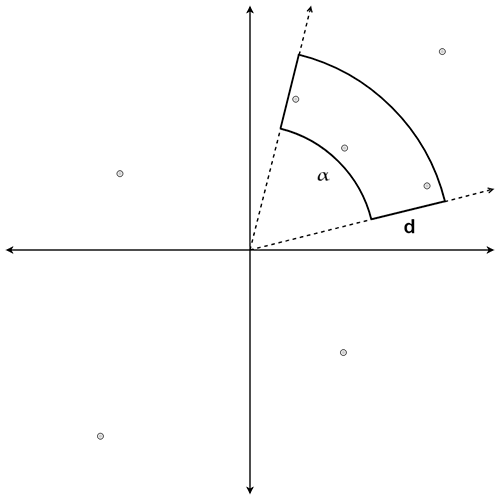
\includegraphics[width=6cm]  {数据结构/扫描线/旋转扫描线pic.jpg}}
\end{figure}
\lstinputlisting{数据结构/扫描线/旋转扫描线.cpp}

\subsubsection{三维求面积交}
\lstinputlisting{数据结构/扫描线/三维求面积交.cpp}


\subsection{可持久化线段树(主席树)}

\subsubsection{静态区间第K小}
\lstinputlisting{数据结构/主席树/静态区间第K小.cpp}

\subsubsection{区间内不同数个数}
\lstinputlisting{数据结构/主席树/区间内不同数个数.cpp}

\subsubsection{树上路径点权第K大}
\lstinputlisting{数据结构/主席树/树上路径点权第K大.cpp}

\subsubsection{区间MEX}
\lstinputlisting{数据结构/主席树/区间MEX.cpp}

\subsection{无旋Treap(FHQ Treap)}
\subsubsection{区间翻转}
\lstinputlisting{数据结构/无旋Treap/fhq_treap.cpp}

\subsubsection{可持久化FHQ}
第一行包含一个正整数$n$,表示操作的总数。\par
接下来$n$行,每行包含三个整数,第$i$行记为${v}_{i}$, ${opt}_i$, $x_i$。\par
$v_i$表示基于的过去版本号,${opt}_i$表示操作的序号,$x_i$表示参与操作的数值。
\lstinputlisting{数据结构/无旋Treap/可持久化FHQ.cpp}


\subsection{树套树}

\subsubsection{带修主席树}
\lstinputlisting{数据结构/树套树/带修主席树.cpp}

\subsubsection{区间修改区间查询第K大([ZJOI2013]K大数查询)}
\lstinputlisting{数据结构/树套树/区间修改区间查询第K大([ZJOI2013]K大数查询).cpp}

\subsection{笛卡尔树}
\subsubsection{建树}
\lstinputlisting{数据结构/笛卡尔树/建树.cpp}


\subsection{动态树LCT}

\subsubsection{lct连链、断链、更改点权、查询链上点权异或和}
\lstinputlisting{数据结构/LCT/lct.cpp}

\subsubsection{树上路径染色([SDOI2011]染色)}
\lstinputlisting{数据结构/LCT/树上路径染色([SDOI2011]染色).cpp}

\subsubsection{SAM+线段树+LCT离线统计区间本质不同字串个数}
时间复杂度:$O(n\log^{2}n+q\log n)$.
\lstinputlisting{数据结构/LCT/SAM+线段树+LCT离线统计区间本质不同字串个数.cpp}

\subsubsection{主席树+LCT在线查询区间连通块个数}
\lstinputlisting{数据结构/LCT/主席树+LCT在线查询区间连通块个数.cpp}

\subsection{KD树}

\subsubsection{平面最近点对}
时间复杂度:单次查询最近点的时间复杂度$O(n).$
\lstinputlisting{数据结构/KD树/平面最近点对.cpp}

\subsubsection{K远点对([CQOI2016])}
已知平面内$N$个点的坐标,求欧氏距离下的第$K$远点对。\par
两个点的欧氏距离为$\sqrt{(x_1-x_2)^{2}+(y_1-y_2)^{2}}$\par
原题数据范围:$N\leq 1e5, 1\leq K\leq 100$\par
时间复杂度:$O(kn\log{n}).$
\lstinputlisting{数据结构/KD树/K远点对.cpp}

\subsubsection{高维空间上的操作}
在一个初始值全为$0$的$n\times n$的二维矩阵上,进行若干次操作,每次操作为以下两种之一:\par
\textbf{1 x y A} 将坐标$(x,y)$上的数加上$A$。\par
\textbf{2 x1 y1 x2 y2} 输出以$(x1, y1)$为左下角,$(x2, y2$为右上角的矩形内(包括矩形边界)的数字和。\par
原题数据范围:$1\leq n \leq 5e5, 1\leq q \leq 2e5$\par
时间复杂度:单次查询时间最优$O(\log{n})$, 最坏$O(\sqrt{n})$。将结论扩展至$k$维,最坏复杂度$O(n^{1-\frac{1}{k}})$
\lstinputlisting{数据结构/KD树/高维空间上的操作.cpp}


\subsection{珂朵莉树/老司机树/ODT}
\subsubsection{set实现珂朵莉树}
\textbf{1 l r x} 将$[l,r]$区间所有数加上$x$\par
\textbf{2 l r x} 将$[l,r]$区间所有数改成$x$\par
\textbf{3 l r x} 输出将$[l,r]$区间从小到大排序后的第$x$个数是的多少(即区间第$x$小,数字大小相同算多次,保证$1\leq x \leq r-l+1$)\par
\textbf{4 l r x y} 输出$[l,r]$区间每个数字的$x$次方的和模$y$的值(即$\sum ^ {r}_{i=l} a_i^x \% y$)\par
时间复杂度:用set实现$O(n\log \log {n})$\par
如果要保证复杂度正确,必须保证数据随机。\par
\lstinputlisting{数据结构/ODT/set实现珂朵莉树.cpp}


\subsection{01字典树}

\subsubsection{路径为点权异或值求最小生成树(CF888G)}
\begin{table}[h]
    \begin{tabular}{ll}
        \hline
        \thead[l]{input} & \thead[l]{output} \\
        \hline
        4  \\ 1 2 3 4 &  8 \\
        \hline       
    \end{tabular}
    \label{bs}
\end{table}
\lstinputlisting{数据结构/01字典树/路径为点权异或值求最小生成树(CF888G).cpp}

\subsubsection{可持久化01字典树}
初始有$n$个数,有$m$个操作:\par
\textbf{1 A x} 添加操作,表示在序列末尾添加一个数 $x$ ,序列的长度 $n+1$\par
\textbf{Q l r x} 询问操作,你需要找到一个位置 $p$ ,满足$l \le p \le r$,使得:$ a[p] \oplus a[p+1] \oplus ... \oplus a[N] \oplus x$最大,输出最大是多少。
\lstinputlisting{数据结构/01字典树/可持久化01字典树.cpp}



\subsection{左偏树(可并堆)}

\subsubsection{左偏树$O(\log n)$}
\lstinputlisting{数据结构/左偏树/LT.cpp}

\subsubsection{带push\_down操作的左偏树子树节点合并([JLOI2015]城池攻占)}
\lstinputlisting{数据结构/左偏树/带push_down操作的左偏树子树节点合并([JLOI2015]城池攻占).cpp}


%================================杂项================================%
\section{杂项}

\subsection{数列归纳}

$f(n) = \frac{(2*n + 1)!}{(n + 1)}$\par
1, 3, 40, 1260, 72576, \par
6652800, 889574400, 163459296000, 39520825344000, 12164510040883200, \par
4644631106519040000, 2154334728240414720000, 1193170003333152768000000, 777776389315596582912000000\par

~\\

$f(n) = \sum_{i=1}^{n} p, p \in prime$\par
转$min_25筛$\par
0, 2, 5, 10, 17, 28, 41, 58, 77, 100, \par
129, 160, 197, 238, 281, 328, 381, 440, 501, 568, \par
639, 712, 791, 874, 963, 1060, 1161, 1264, 1371, 1480, \par
1593, 1720, 1851, 1988, 2127, 2276, 2427, 2584, 2747, 2914, \par
3087, 3266, 3447, 3638, 3831, 4028, 4227, 4438, 4661, 4888\par
\par



\subsection{全1矩阵个数(51nod1291)}
\begin{table}[h]
    \begin{tabular}{ll}
        \hline
        \thead[l]{input} & \thead[l]{output} \\
        \hline
        3 3 & \\
        011 & 6 3 0\\
        110 & 3 1 0\\
        100 & 1 0 0\\
        \hline       
    \end{tabular}
    \label{bs}
\end{table}
\lstinputlisting{杂项/全1矩阵个数(51nod1291).cpp}

\subsection{华容道}
\lstinputlisting{其它/华容道.cpp}

\subsection{希尔伯特曲线}
\begin{figure}[htb] 
 \center{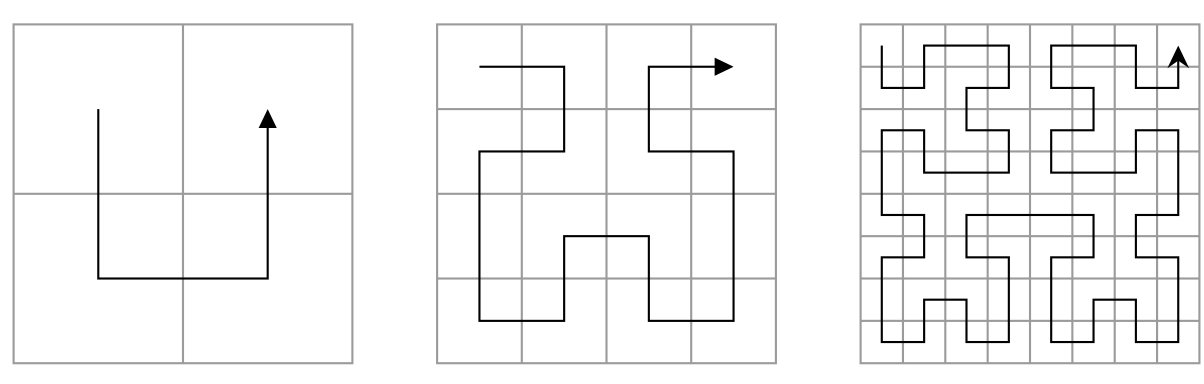
\includegraphics[width=15cm]  {其它/希尔伯特曲线_pic.png}} 
 \end{figure}
\lstinputlisting{其它/希尔伯特曲线.cpp}

\subsection{非整数希尔伯特曲线}
\lstinputlisting{其它/非整数希尔伯特曲线.cpp}

\subsection{约瑟夫环}
\subsubsection{一般方法}
\lstinputlisting{其它/约瑟夫环/一般方法.cpp}
\subsubsection{函数图像解}
\lstinputlisting{其它/约瑟夫环/函数图像解.cpp}

%==============================计算几何==============================%
\section{计算几何}


%==============================习题整理==============================%
\section{习题整理}

\subsection{可重边集的点能否和当前询问边构成三角形(20牛客2H)(动态点开线段树)}
\begin{table}[h]
    \begin{tabular}{ll}
        \hline
        \thead[l]{input} & \thead[l]{output} \\
        \hline
        8   & \\
        1 1 & \\
        3 1 & No \\
        1 1 & \\
        3 2 & No \\
        3 1 & Yes \\
        1 2 & \\
        2 1 & \\
        3 1 & No \\
        \hline       
    \end{tabular}
    \label{bs}
\end{table}
\lstinputlisting{习题整理/可重边集的点能否和当前询问边构成三角形(20牛客2H)(动态点开线段树).cpp}

\subsection{左偏树离线处理查询成立最多数(HDU5575)}
$0$代表没有水,$1$代表有水\par
\begin{table}[h]
    \begin{tabular}{ll}
        \hline
        \thead[l]{input} & \thead[l]{output} \\
        \hline
        3 4   & 3 \\
        3 4 & \\
        1 3 1 & \\
        2 1 0 & \\
        2 2 0 & \\
        3 3 1 & \\
        \hline       
    \end{tabular}
    \label{bs}
\end{table}
\lstinputlisting{习题整理/左偏树离线处理查询成立最多数(HDU5575).cpp}

%==============================st1vdy计算几何==============================%
\section{st1vdy计算几何}
\lstinputlisting{st1vdy.cpp}

\end{document}